\documentclass[tikz,border=5mm]{standalone}
\usetikzlibrary{arrows, positioning, shapes, fit}

\begin{document}
    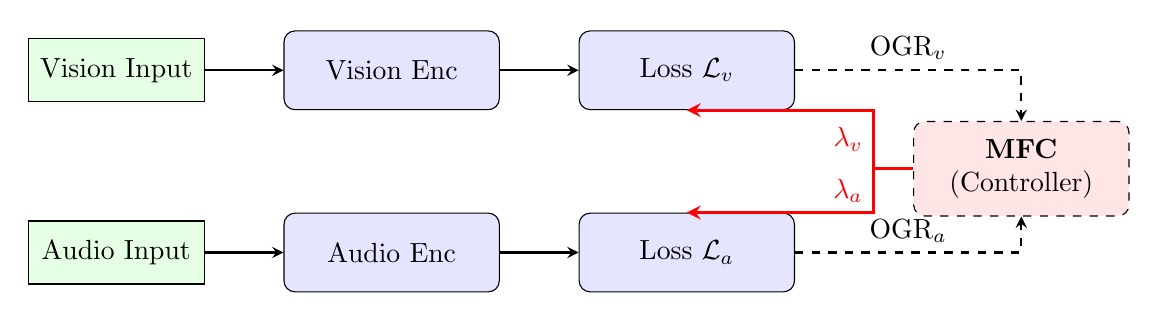
\begin{tikzpicture}[node distance=1.2cm, >=stealth, auto,
        block/.style={rectangle, draw, fill=blue!10, text width=2.5cm, text centered, rounded corners, minimum height=1.0cm},
        sensor/.style={rectangle, draw, fill=green!10, text width=2.0cm, text centered, minimum height=0.8cm},
        control/.style={rectangle, draw, fill=red!10, text width=2.5cm, text centered, rounded corners, minimum height=1.2cm, dashed}
        ]
        % Nodes
        \node [sensor] (vis) {Vision Input};
        \node [block, right=1cm of vis] (encv) {Vision Enc};
        \node [block, right=1cm of encv] (lossv) {Loss $\mathcal{L}_v$};

        \node [sensor, below=1.5cm of vis] (aud) {Audio Input};
        \node [block, right=1cm of aud] (enca) {Audio Enc};
        \node [block, right=1cm of enca] (lossa) {Loss $\mathcal{L}_a$};
        
        \node [control, right=1.5cm of lossv, yshift=-1.25cm] (mfc) {\textbf{MFC} \\ (Controller)};
        
        % Edges
        \draw[->, thick] (vis) -- (encv);
        \draw[->, thick] (encv) -- (lossv);
        
        \draw[->, thick] (aud) -- (enca);
        \draw[->, thick] (enca) -- (lossa);
        
        % Feedback
        \draw[->, dashed, thick] (lossv) -| node[near start, above] {OGR$_v$} (mfc);
        \draw[->, dashed, thick] (lossa) -| node[near start, above] {OGR$_a$} (mfc);
        
        \draw[->, red, very thick] (mfc.west) -- ++(-0.5,0) |- node[near start, left] {$\lambda_v$} (lossv.south);
        \draw[->, red, very thick] (mfc.west) -- ++(-0.5,0) |- node[near start, left] {$\lambda_a$} (lossa.north);
        
    \end{tikzpicture}
\end{document}
